%---------- Inleiding ---------------------------------------------------------

% TODO: Is dit voorstel gebaseerd op een paper van Research Methods die je
% vorig jaar hebt ingediend? Heb je daarbij eventueel samengewerkt met een
% andere student?
% Zo ja, haal dan de tekst hieronder uit commentaar en pas aan.

% \paragraph{Opmerking}

% Dit voorstel is gebaseerd op het onderzoeksvoorstel dat werd geschreven in het
% kader van het vak Research Methods dat ik vorig academiejaar heb
% uitgewerkt.

\section{Inleiding}%
\label{sec:inleiding}

\subsection{Overzicht}

TVH is een retail bedrijf dat zich focust op de verkoop van onderdelen binnen de logistieke sector. 
De hoofdzetel is gevestigd in Waregem, België en heeft een eigen IT-afdeling.
Bedrijven zoals TVH hebben verschillende domeinen en subdomeinen met specifieke doeleinden binnen de organisatie. 
Deze bachelorproef speelt zich af binnen het domein "warehousing", dat instaat voor de opslag en beheer van goederen. 
Warehousing in TVH omvat verschillende magazijnen, waaronder automatische magazijnen die worden aangestuurd door PLC's en een WMS.
Een van de magazijnen die hier in deze paper in aanmerking komt is de oudste binnen TVH. 
Dat automatisch magazijn wordt aangedreven door een PLC (Programmable Logic Controller) 
van Vanderlanden en bestaat uit een conveyor systeem met een ASRS (Automatic Storage and Retrieval System).
De PLC stuurt informatie over het systeem en data van bakken die op het systeem routeren naar het WMS (Warehouse Management System). 
Dit WMS is geschreven in Progress 4GL-code en maakt deel uit van het monolithische ERP-pakket dat door TVH is geïmplementeerd. 
De PLC ontvangt bijvoorbeeld een taak om een bak naar een bepaalde bestemming te sturen. 
De volledige opzet van dit systeem wordt later besproken.

% hook
Om deze taken te kunnen uitvoeren, wordt gebruikgemaakt van één of meerdere \emph{services}. 
In de IT-terminologie staat deze opstelling bekend als \emph{“Service Oriented Architecture” (SOA)}, 
die steeds populairder wordt vanwege de voordelen voor \emph{flexibiliteit} en \emph{schaalbaarheid} \autocite{Bellemare2020}.

Door deze onderlinge afhankelijkheid moeten services met elkaar kunnen communiceren. 
Om dit mogelijk te maken, zijn verschillende \emph{messaging-systemen} beschikbaar op de markt, 
elk met hun eigen eigenschappen en toepassingen.
\newline 

TVH heeft een snelle groei doorgemaakt zonder algemene afspraken te maken rond het gebruik van messaging systemen. 
Dit heeft geresulteerd in de implementatie van verschillende messaging systemen, waardoor er een diversiteit aan oude en moderne technologieën in gebruik is. 
\newline 
\newline
\newline

\subsection{Probleemstelling}
De OS op de server die verantwoordelijk is voor de communicatie tussen WMS en PLC van het oudste automatisch magazijn wordt niet ondersteund.
Dit kan gevolgen hebben op het gebied van veiligheidsrisico's en moet daarom vervangen worden.
De server draait momenteel op CentOS 6.6 als besturingssysteem en zal worden vervangen door Red Hat.
Het vervangen van de server valt buiten de scope van dit onderzoek. 
Omdat de software op de oude server niet op modernere besturingssystemen kan worden geïnstalleerd, 
moeten we zoeken naar een alternatief.
\newline

Volgende nadelen van verouderde messaging systemen doen zich voor: 
De onderhoudskosten, waardoor mensen in de firma specifiek opgeleid moeten worden om deze te onderhouden. 
Beveilgingsrisico's, cybercriminelen richten zich vaak op verouderde software, omdat de kwetsbaarheden publiekelijk bekend zijn en niet meer worden aangepakt.
Verouderde software heeft een hogere kans op uitval, wat leidt tot hogere kosten door verlies van productiviteit en herstelwerkzaamheden.
\newline 

\subsection{Onderzoeksdoelstelling}
Het doel van dit onderzoek is om te bepalen welk messaging systeem het meest geschikt is voor de vervanging van de huidige SonicMQ,
die gebruikt wordt voor de communicatie tussen WMS en PLC. 
Hierbij moet er rekening gehouden worden met de niet-functionele vereisten,
zoals flexibiliteit, performantie, beveiliging en integratiemogelijkheden.
Naast de vergelijkende studie moet er ook gekeken worden wat de kosten en de inspanningen zijn 
voor het integreren van een gekozen messaging systeem. 
\newline 

\newpage

\subsection{Onderzoeksvraag en deelvragen}
Welke \emph{messaging technologieën} zijn het meest geschikt om het verouderde SonicMQ-systeem te vervangen 
en de communicatie tussen het Warehouse Management System (WMS) en de Programmable Logic Controllers (PLC’s) 
in het automatische magazijn te garanderen?

Enkele cruciale deelvragen met betrekking tot de hoofdvraag:
\begin{enumerate}
  \item Waarom is SonicMQ niet ondersteund op een Red Hat OS?
  \item Welke messaging systemen zijn er beschikbaar?
  \item Waarom is een weloverwogen keuze van essentieel belang?
  \item Wat is de inspanning om een gekozen technologie te implementeren?
  \item Wat zijn de non-functional requirements van de bestaande service?
  \item Welk messaging systeem is een weloverwogen keuze?
\end{enumerate}

\subsection{Opbouw van het onderzoek}
Eerst zal de literatuurstudie in hoofdstuk \ref{sec:literatuurstudie} een breder inzicht geven in volgende topics.
\begin{enumerate}
  \item Wat is een PLC en wat doet het
  \item Wat is een WMS en waarvoor staat het
  \item Wat zijn messaging systemen
  \item Wat is synchrone en asynchrone communicatie
  \item Wat is de huidige setup tussen WMS en PLC
  \item Waarom is CentOS 6 niet veilig
\end{enumerate}

Hoofdstuk \ref{sec:methodologie} beschrijft de methodologie en de stappen die nodig zijn om dit onderzoek te ondersteunen
en te leiden tot een rapport met aanbevelingen.
\newline

In hoofdstuk \ref{sec:verwachte-resultaten} worden de verwachte resultaten besproken, gevolgd door 
hoofdstuk \ref{sec:discussie-conclusie} met de verwachte conclusie van dit onderzoek.

\bigskip


%---------- Stand van zaken (State-of-the-art)---------------------------------------------------

\section{Literatuurstudie}%
\label{sec:literatuurstudie}

% Hier beschrijf je de \emph{state-of-the-art} rondom je gekozen onderzoeksdomein, d.w.z.\ een inleidende, doorlopende tekst over het onderzoeksdomein van je bachelorproef. Je steunt daarbij heel sterk op de professionele \emph{vakliteratuur}, en niet zozeer op populariserende teksten voor een breed publiek. Wat is de huidige stand van zaken in dit domein, en wat zijn nog eventuele open vragen (die misschien de aanleiding waren tot je onderzoeksvraag!)?

% Je mag de titel van deze sectie ook aanpassen (literatuurstudie, stand van zaken, enz.). Zijn er al gelijkaardige onderzoeken gevoerd? Wat concluderen ze? Wat is het verschil met jouw onderzoek?

% Verwijs bij elke introductie van een term of bewering over het domein naar de vakliteratuur, bijvoorbeeld~\autocite{Hykes2013}! Denk zeker goed na welke werken je refereert en waarom.

% Draag zorg voor correcte literatuurverwijzingen! Een bronvermelding hoort thuis \emph{binnen} de zin waar je je op die bron baseert, dus niet er buiten! Maak meteen een verwijzing als je gebruik maakt van een bron. Doe dit dus \emph{niet} aan het einde van een lange paragraaf. Baseer nooit teveel aansluitende tekst op eenzelfde bron.

% Als je informatie over bronnen verzamelt in JabRef, zorg er dan voor dat alle nodige info aanwezig is om de bron terug te vinden (zoals uitvoerig besproken in de lessen Research Methods).

% Voor literatuurverwijzingen zijn er twee belangrijke commando's:
% \autocite{KEY} => (Auteur, jaartal) Gebruik dit als de naam van de auteur
%   geen onderdeel is van de zin.
% \textcite{KEY} => Auteur (jaartal)  Gebruik dit als de auteursnaam wel een
%   functie heeft in de zin (bv. ``Uit onderzoek door Doll & Hill (1954) bleek
%   ...'')

% Je mag deze sectie nog verder onderverdelen in subsecties als dit de structuur van de tekst kan verduidelijken.

\bigskip
 
% \subsection{Definitie van Domein}
% TVH is een bedrijf dat verschillende domeinen met subdomeinen bevat.
% Het woord domein in de bedrijfscontext is een probleemgebied waar een bedrijf zich op richt en oplossingen voor biedt. 
% De firma heeft als hoofddomein e-commerce en omvat alle aspecten van hun online retailactiviteiten, 
% zoals het beheren van producten, het verwerken van bestellingen, klantenservice, marketing en logistiek.
% \newline 

% Een domein bevat subdomeinen die elk gericht zijn op een specifieke subset zoals bijvoorbeeld ``Warehousing''.
% Dit subdomein richt zich specifiek op het beheren van goederen, met ondersteuning van het toevoegen, bewerken en verwijderen van producten, 
% evenals het bijhouden van voorraadniveaus.
% \newline 

% Een subdomein kan dus worden beschouwd als een stukje van het domein, 
% dat net als het domein zelf behoort tot het probleemgebied.   
% Terwijl een domein een breed probleemgebied beschrijft, bevat een subdomein een specifieke afbakening, genaamd \emph{bounded context}.
% Dit maakt het mogelijk om \emph{services} binnen deze afbakening te ontwikkelen en te beheren \autocite{Bellemare2020}.

%\subsection{Soorten communicatie}
% file:///C:/Data/Downloads/IJMECS-V12-N2-5.pdf
 
\subsection{Synchroon vs. asynchroon}
Services communiceren zowel \emph{synchroon} als \emph{asynchroon} en spelen deze benaderingen een cruciale rol, 
elk met hun eigen voor- en nadelen. \emph{Synchrone microservices} werken volgens een direct 
afhankelijkheidsmodel, omdat services met elkaar communiceren in een vraag-antwoordpatroon. 
Deze synchrone communicatie kan leiden tot ingewikkelde onderlinge afhankelijkheden, vertragingen en complexiteiten bij het debuggen 
van de logica. Bovendien wordt het schalen van synchrone microservices uitdagend, 
aangezien de schaalbaarheid van één service sterk afhankelijk is van andere services die het gebruikt \autocite{Bellemare2020}. 
\newline

Daartegenover bieden \emph{asynchrone microservices} een reeks voordelen. Ze bieden grotere schaalbaarheid, technologische 
flexibiliteit en aanpassingsvermogen aan veranderende zakelijke vereisten. 
In plaats van de synchrone manier van communicatie zijn \emph{asynchrone microservices} 
gemakkelijker te herstructureren en te onderhouden. 
Ze vergemakkelijken \emph{continuous delivery} door hun onafhankelijkheid omdat de communicatie 
met een \emph{messaging systeem} opgevangen wordt. Hun verminderde afhankelijkheden en 
geïsoleerde karakter maken het testen relatief eenvoudiger en robuuster.
Het enige grote nadeel in asynchrone communicatie is \emph{error handling}, 
omdat dit niet opgevangen kan worden door de verzendende partij.
\newline

\begin{figure}[H]
  \centering
  \includegraphics[width=.5\textwidth]{../voorstel/img/synchronous_vs_async_calls.png}
  \caption{\label{fig:img}Synchronous versus asynchronous communication \autocite[figure 14 -- 13]{MarkRichards2021}.}
\end{figure}

In praktische termen is het vinden van de juiste balans tussen synchrone en \emph{asynchrone microservices} cruciaal, 
afhankelijk van de specifieke behoeften van een organisatie en de aard van haar bedrijfsprocessen. 
Een hybride aanpak waarin beide architecturen naast elkaar bestaan en elkaar aanvullen blijkt vaak de meest effectieve strategie te zijn. 
Deze aanpak stelt organisaties in staat om de sterke punten van zowel synchrone als asynchrone modellen te benutten, 
waardoor flexibiliteit, schaalbaarheid en onderhoudsgemak worden gegarandeerd in complexe \newline IT-landschappen.
In deze paper ligt de focus op \emph{asynchrone communicatie} voor het gebruik van \emph{messaging systemen}.
\newline

\subsection{Overzicht Messaging Systeem}
Messaging systemen hebben dus een asynchrone werking en vallen onder \newline \emph{Inter-Process Communication (IPC)}. 
Deze systemen zijn \emph{socket-based} en maken gebruik van \emph{message queuing}, waarbij het de \emph{publish-subscribe} of de \emph{point-to-point} methodiek gebruikt \autocite{Dinari2020}. 
\newline
Een socketverbinding maakt gebruik van een endpoint gespecificeerd met een IP-adres en een \newline poortnummer, 
waarmee twee autonome processen verbonden zijn, hetzij op dezelfde, hetzij op verschillende machines.
\newline
\emph{Message Queuing} gebruikt deze manier van verbinden en maakt het voor applicaties mogelijk om asynchroon 
te communiceren zonder te moeten wachten op een antwoord van de ontvanger. 
Er zijn twee methodieken in deze systemen. 
\newline

De eerste methodiek is \emph{publish-subscribe}, waarbij de zender, genaamd \emph{publisher} niet verantwoordelijk is voor het beheer 
en het rechtstreeks verzenden van de berichten naar specifieke ontvangers, die \emph{subscribers} of abonnees worden genoemd. 
In plaats daarvan worden berichten door het messaging systeem of broker geclassificeerd en ter 
beschikking gesteld van de subscribers die ingetekend hebben op berichten uit een specifieke klasse.
Vervolgens ontvangen \emph{subscribers} berichten uit de klassen die voor hen interessant zijn, zonder dat ze kennis hebben van de \emph{publishers}.
Met het \emph{publish-subscribe-model} specificeert de afzender nooit expliciet de ontvanger,
hij weet zelfs niet of er wel of geen ontvanger bestaat.
\newline

\begin{figure}[h]
  \centering
  \includegraphics[width=.4\textwidth]{../voorstel/img/fig1-publish-subscribe.png}
  \caption{\label{fig:img}Publisher-Subscriber system\autocite{Sharvari2019}.}
\end{figure}

In dit model ontvangen \emph{subscribers} slechts een subset van de totale gepubliceerde berichten. 
Het proces van het selecteren en verwerken van de berichten wordt filtering genoemd. 
Er zijn twee vormen van filtering: op basis van onderwerp (topic) en op basis van inhoud (content).
\newline

In een op \emph{topic} gebaseerd systeem worden berichten geplaatst in \emph{topics} wat logische kanalen zijn.
\emph{Subscribers} ontvangen berichten van de \emph{topics} waarop ze zich hebben geabonneerd.
Alle \emph{subscribers} ontvangen dezelfde berichten uit dezelfde \emph{topics}. 
Deze methode zorgt voor een \emph{one-to-many} vorm van communicatie.
\newline

De tweede methodiek genaamd point-to-point gebruikt \emph{queuing} waarbij de \emph{producer} berichten plaatst in een specifieke queue, 
waarna een \emph{consumer} de berichten uitleest in een sequentiele volgorde. 
Met andere woorden, een bericht wordt slechts aan één \emph{consumer} bezorgt.

\subsection{Wat is een PLC}
Een PLC (Programmable Logic Controller) is een industriële computer die wordt gebruikt voor het automatiseren van machines en processen \autocite{Bolton2015}. 
Het is ontworpen om robuust te zijn en betrouwbaar te functioneren in industriële omgevingen zoals fabrieken, 
waar het vaak wordt gebruikt om mechanische apparatuur, zoals transport systemen of liften van een automatisch magazijn te besturen.

\subsection{Wat is een WMS}
Warehouse managementsystemen (WMS) zijn softwaretoepassingen die bedrijven in staat stellen om magazijnactiviteiten te beheren en te controleren, 
waaronder voorraadbeheer, orderverwerking en transportbeheer. 
Warehouse managementsystemen (WMS) vormen een essentieel onderdeel van moderne magazijnactiviteiten \autocite{Rana2023}. \newline

Een aantal onderzoeksvragen uit de probleemstelling dat deels kan worden beantwoord:

\begin{enumerate}

\item \textbf{Waarom is een weloverwogen keuze van essentieel belang?}
  \begin{itemize}
      \item Een weloverwogen keuze is essentieel omdat het huidige communicatie systeem inefficiëntie kan veroorzaaken en niet op modernere systemen 
      kan worden geïnstalleerd worden. Door zorgvuldig te kiezen kan dit probleem opgelost worden en een 
      efficiënter IT-landschap creëren.
  \end{itemize}

\item \textbf{Wat is de inspanning om een gekozen technologie te implementeren?}
  \begin{itemize}
      \item De inspanning om een gekozen technologie te implementeren kan variëren afhankelijk van de specifieke systeemvereisten, 
      de non-functional requirements en de beschikbare middelen binnen de organisatie. Dit kan onder meer het configureren, 
      aanpassen en integreren van de gekozen technologie omvatten, evenals het trainen van personeel en het uitvoeren van migraties van 
      bestaande systemen.
  \end{itemize}
\end{enumerate}

\newpage

%---------- Methodologie ------------------------------------------------------
\section{Methodologie}%
\label{sec:methodologie}

% Hier beschrijf je hoe je van plan bent het onderzoek te voeren. Welke onderzoekstechniek ga je toepassen om elk van je onderzoeksvragen te beantwoorden? Gebruik je hiervoor literatuurstudie, interviews met belanghebbenden (bv.~voor requirements-analyse), experimenten, simulaties, vergelijkende studie, risico-analyse, PoC, \ldots?

% Valt je onderwerp onder één van de typische soorten bachelorproeven die besproken zijn in de lessen Research Methods (bv.\ vergelijkende studie of risico-analyse)? Zorg er dan ook voor dat we duidelijk de verschillende stappen terug vinden die we verwachten in dit soort onderzoek!

% Vermijd onderzoekstechnieken die geen objectieve, meetbare resultaten kunnen opleveren. Enquêtes, bijvoorbeeld, zijn voor een bachelorproef informatica meestal \textbf{niet geschikt}. De antwoorden zijn eerder meningen dan feiten en in de praktijk blijkt het ook bijzonder moeilijk om voldoende respondenten te vinden. Studenten die een enquête willen voeren, hebben meestal ook geen goede definitie van de populatie, waardoor ook niet kan aangetoond worden dat eventuele resultaten representatief zijn.

% Uit dit onderdeel moet duidelijk naar voor komen dat je bachelorproef ook technisch voldoen\-de diepgang zal bevatten. Het zou niet kloppen als een bachelorproef informatica ook door bv.\ een student marketing zou kunnen uitgevoerd worden.

% Je beschrijft ook al welke tools (hardware, software, diensten, \ldots) je denkt hiervoor te gebruiken of te ontwikkelen.

% Probeer ook een tijdschatting te maken. Hoe lang zal je met elke fase van je onderzoek bezig zijn en wat zijn de concrete \emph{deliverables} in elke fase?

Het volgende stappenplan zal helpen om de vergelijkende studie op een verfijnde manier uit te voeren.
Eerst worden de requirements rond messaging systemen per subdomein opgelijst aan de hand van diepte interviews 
met de ontwikkelaars en de software architects. 
Deze requirements zullen ook duidelijk maken welke criteria exact van belang zijn.
Daarnaast worden de verschillende soorten messaging systemen die beschikbaar zijn op de markt opgezocht, bestudeerd en opgelijst in een longlist.
Voor het bekomen van een shortlist zal de longlist onderworpen worden aan eerder opgestelde criteria.
\newline

Tijdens deze studie worden een aantal testen opgesteld om na te gaan of de gekozen technologieën in de shortlist voldoen aan de non-functional requirements.
Na het uitvoeren van de testen zal een uitgebreide analyse uitwijzen welk systeem het meest optimaal is binnen de firma.

\subsection{Stappen plan}

\begin{figure}[htbp]
  \centering
  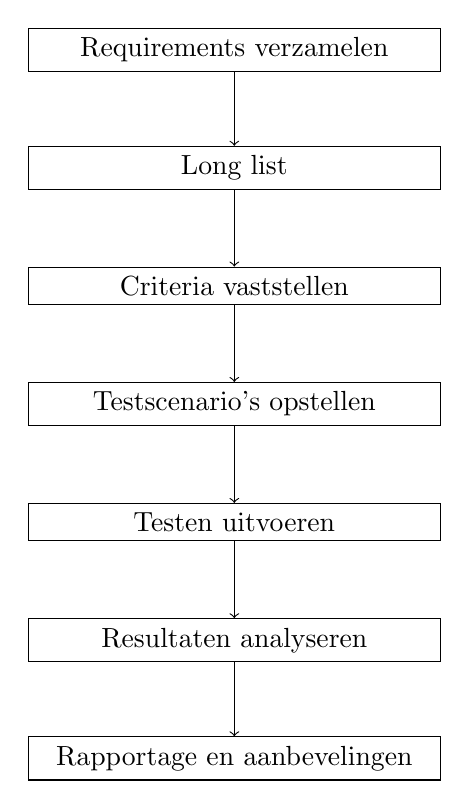
\begin{tikzpicture}[node distance=1.5cm]
      % Nodes
      \node (start) [rectangle, draw, text width=5cm, align=center] {Requirements verzamelen};
      \node (longlist) [rectangle, draw, below of=start, text width=5cm, align=center] {Long list};
      \node (criteria) [rectangle, draw, below of=longlist, text width=5cm, align=center] {Criteria vaststellen};
      \node (testscenario) [rectangle, draw, below of=criteria, text width=5cm, align=center] {Testscenario's opstellen};
      \node (testen) [rectangle, draw, below of=testscenario, text width=5cm, align=center] {Testen uitvoeren};
      \node (analyseren) [rectangle, draw, below of=testen, text width=5cm, align=center] {Resultaten analyseren};
      \node (rapportage) [rectangle, draw, below of=analyseren, text width=5cm, align=center] {Rapportage en aanbevelingen};

      % Arrows
      \draw [->] (start) -- (longlist);
      \draw [->] (longlist) -- (criteria);
      \draw [->] (criteria) -- (testscenario);
      \draw [->] (testscenario) -- (testen);
      \draw [->] (testen) -- (analyseren);
      \draw [->] (analyseren) -- (rapportage);
  \end{tikzpicture}
  \caption{Stappen van het onderzoeksproces}
  \label{fig:flowchart}
\end{figure}


\bigskip

\subsection{Tijdlijn}

De volgende tijdlijn geeft naar schatting een overzicht van wanneer elk onderdeel zal plaatsvinden en hoeveel tijd elk onderdeel in beslag zal nemen. 
Er zijn vier dagen per maand beschikbaar waarop acht uur kan worden gewerkt aan dit onderzoek.

\newcommand{\ytl}[2]{
  \parbox[b]{8em}{\hfill{\color{cyan}\bfseries\sffamily #1}~$\cdots\cdots$~}\makebox[0pt][c]{$\bullet$}\vrule\quad \parbox[c]{4.5cm}{\vspace{7pt}\color{red!40!black!80}\raggedright\sffamily #2.\\[7pt]}\\[-3pt]
}

\begin{figure}[htbp]
  \centering  
  \rule{\linewidth}{1pt}
  \ytl{Okt, 2 dagen}{Requirements verzamelen -- Criteria vaststellen}
  \ytl{Okt, 2 dagen}{Long list naar Short list}
  \ytl{Nov, 1 dag}{Opstellen testscenario's}
  \ytl{Nov, 2 dagen}{Testen}
  \ytl{Dec, 2 dagen}{Analyseren resultaten}
  \ytl{Dec, 2 dagen}{Rapportage}
  \rule{\linewidth}{1pt}
  \caption{Tijdlijn onderzoek}
  \label{fig:timeline}
\end{figure}

 
\subsection{Requirements verzamelen}
In deze stap worden de criteria opgenomen om de longlist in een latere fase te kunnen filteren.
Door documentatie op te zoeken kan een lijst met criteria gecategoriseerd worden volgens de non-functional requirements.

\subsection{Evaluatiecriteria vaststellen}
We stellen criteria vast om de verschillende messaging systemen te kunnen evalueren. 
Deze criteria moeten relevant zijn voor de behoeften en vereisten van het bedrijf, en kunnen onder meer omvatten:
\begin{itemize}
  \item Performantie: Snelheid, schaalbaarheid
  \item Betrouwbaarheid: Transactiemogelijkheden, error handling
  \item Beveiliging: Encryptie, authenticatie
  \item Integratiemogelijkheden: Compatibiliteit \newline met bestaande systemen, API-ondersteuning
  \item Onderhoudsvriendelijkheid: Implementatiegemak, onderhoudsvereisten, documentatie
  \item Kosten: Licentiekosten, onderhoudskosten
\end{itemize}

\subsection{Long list naar Short list}
Identificeren van een selectie messaging systemen die op de markt beschikbaar zijn en relevant zijn voor de communicatie tussen 
het WMS en de PLC's (Long list), zodat deze in een latere fase kunnen worden beoordeeld aan de hand van specifieke criteria, 
met als doel een shortlist op te stellen van twee technologieën die verder zullen worden opgenomen in de proof of concept (PoC).

\subsection{Opstellen van Testscenario's}
De volgende testscenario's helpen bij dit onderzoek om de prestaties en functionaliteit van de messaging systemen 
objectief te beoordelen.

\begin{itemize}
  \item Versturen en ontvangen van berichten met verschillende grootten en frequenties.
  \item Testen van de beveiligingsmechanismen van het systeem.
  \item Evalueren van de integratiemogelijkheden.
 \end{itemize}

\subsection{Uitvoeren van de testen}
Testen worden uitgevoerd in een afgeschermde omgeving met behulp van tooling zoals Gatling.
Dit is een tool die wordt gebruikt voor performantie testen.
Deze aanpak zal zorgen voor gedetailleerde rapporten over de prestaties van elke messaging technologie onder verschillende belastingniveaus. 
Daarnaast gaan integratiemogelijkheden met monitoring programma's zoals Elasticsearch worden onderzocht.

\subsection{Analyseren en Vergelijken van Resultaten}
De resultaten worden opgenomen per messaging systeem in een beslissingsmatrix om een vergelijking te kunnen uitvoeren. 
Door scores te geven op basis van een vastgestelde schaal kan er objectief een oordeel worden gemaakt.

\subsection{Rapportage van Resultaten en Aanbevelingen}
De rapportering zal een beslissingsmatrix bevatten waarin twee uiteenlopende use-cases met behulp van de 
matrix met elkaar worden vergeleken.

%---------- Verwachte resultaten ----------------------------------------------
\section{Verwacht resultaat, conclusie}%

\label{sec:verwachte-resultaten}

% Hier beschrijf je welke resultaten je verwacht. Als je metingen en simulaties uitvoert, kan je hier al mock-ups maken van de grafieken samen met de verwachte conclusies. Benoem zeker al je assen en de onderdelen van de grafiek die je gaat gebruiken. Dit zorgt ervoor dat je concreet weet welk soort data je moet verzamelen en hoe je die moet meten.

% Wat heeft de doelgroep van je onderzoek aan het resultaat? Op welke manier zorgt jouw bachelorproef voor een meerwaarde?

% Hier beschrijf je wat je verwacht uit je onderzoek, met de motivatie waarom. Het is \textbf{niet} erg indien uit je onderzoek andere resultaten en conclusies vloeien dan dat je hier beschrijft: het is dan juist interessant om te onderzoeken waarom jouw hypothesen niet overeenkomen met de resultaten.

Het onderzoek zal het meest optimale messaging systemen identificeren.
Testen gaan meer inzichten bieden bij het beoordelen van de prestaties, betrouwbaarheid, 
schaalbaarheid, beveiliging, onderhoudbaarheid, compatibiliteit, kosten en gebruikerservaring van elke technologie.
\newline

Tot slot zal het onderzoek dus resulteren in aanbevelingen van verschillende technologieën die het meest geschikt zijn
in de vorm van een beslissingsmatrix. 
Deze aanbevelingen gaan dus gebaseerd zijn op een grondige analyse van de non-functional requirements 
door onderzoek en testen.


\section{Discussie, verwachte conclusie}%
\label{sec:discussie-conclusie}

Het afleveren van de beslissingsmatrix kan helpen bij de besluitvorming bij management om de efficiëntie, schaalbaarheid en integratie van de IT-infrastructuur te verbeteren
en de kosten en complexiteit te verminderen. 
